%%%%%%%%%%%%%%%%%%%%%%%%%%%%%%%%%%%%%%%%%%%%%%%%%
%%%%%%%%%%%% chap: Related Work%%%%%%%%%%%%%%%%%
%%%%%%%%%%%%%%%%%%%%%%%%%%%%%%%%%%%%%%%%%%%%%%%%%

\chapter{Related Work}\label{chapter:chap3}

\section{Similar Applications}\label{sect:similar applications}

\begin{wrapfigure}{r}{0.4\textwidth} 
    \centering
    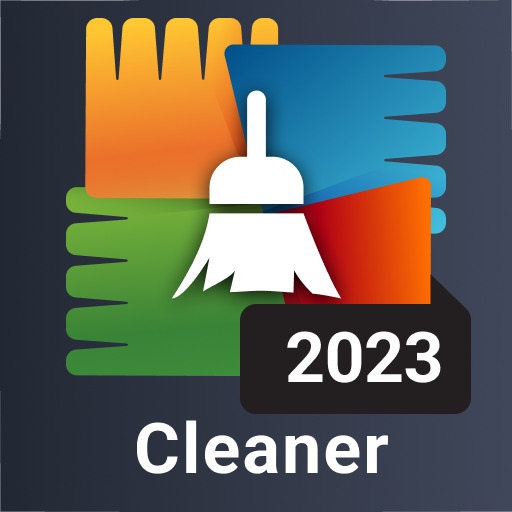
\includegraphics[width=0.4\textwidth]{avg.png}
\end{wrapfigure}

\textbf{1. AVG Cleaner}

\textbf{Developer}: AVG Mobile

\textbf{Description}: AVG is a mobile cleaning tool designed to delete junk files from the phones' storage.

\textbf{Characteristics}:

• \textbf{App analyzer}: The application will identify applications that could be causing mobile data to drain faster;

• \textbf{App remover}: The app can has options for app removal;

• \textbf{Junk cleaner}: The application can delete junk and leftover files;

\textbf{Data security}:

• This application may share data with third parties;

• This application may collect these types of data (Location, Personal info and 3 others);

• Data is encrypted in transit;

• Data can be deleted.\newline

\begin{wrapfigure}{r}{0.4\textwidth} 
    \centering
    
\includegraphics[width=0.4\textwidth]{app2.png}
\end{wrapfigure}

\noindent 
\textbf{2. Phone Cleaner - Cache Clean}

\textbf{Developer}: Games Tree

\textbf{Description}: Phone cleaner is a cleaning app for an Android device and has the following characteristics: file cleaning capabilities, it can cool the CPU, a built-in application manager, and battery-saving functions.

\textbf{Characteristics}:

• \textbf{Cache Cleaner}: The app can clean apps or residual data, such as cache memory;

• \textbf{Storage Cleaner}: This function scans the phone for data to delete and free up space so it can increase the phone's performance;

• \textbf{CPU Cooling}: The app can cool the CPUs temperature and improve its performance;

• \textbf{Battery saving actions}: Another function of the app is the disabling of power-consuming apps;

• \textbf{Notification cleaning functions}: The last function of the app is its notification cleaning capabilities;

\textbf{Data security}:

• No data was collected;

• Data will be encrypted during transit;

• The user can request the data to be deleted;

• No data is shared with third parties.\newline

\begin{wrapfigure}{r}{0.4\textwidth} 
    \centering
    
\includegraphics[width=0.4\textwidth]{app3.png}
\end{wrapfigure}

\noindent 
\textbf{3. CCleaner – Phone Cleaner }

\textbf{Developer}: Piriform

\textbf{Description}: CCleaner helps you remove junk messages from your Android phone. This Android cleaning app clears your browser history, app cache, and clipboard contents. This Android device cleaner also helps to boot faster and provide better performance.

\textbf{Characteristics}:

• The app can clean cache memory, browser memory, and much more;

• Storage cleaning: The app can also analyze storage space and delete unwanted and residual data to boost performance;

• Application hibernation function, which allows the app to keep apps closed until opened manually;

• Ram boosting functions;

• Increases performance and battery life;

• Analyzes the impact of applications;

• Optimizes the storage of photos;

• Monitors the system.

\textbf{Data security}:

• The application may send different types of data to third parties;

• The application may collect the following types of data (Location, Personal Information);

• Data will be encrypted during the transmission period;

• The data can be deleted at request.\newline

\newpage
\begin{wrapfigure}{r}{0.4\textwidth} 
    \centering
    
\includegraphics[width=0.4\textwidth]{1tapcleaner.png}
\end{wrapfigure}

\noindent 
\textbf{4. 1TapCleaner }

\textbf{Developer}: Sam Lu

\textbf{Description}: 1-Tab Cleaner has the ability to clear caches, search histories, and defaults.

\textbf{Characteristics}:

• The app can clean the cache memory;

• Another characteristic is the creation of a list of default apps and the clearing of their selected defaults;

• The application can also clear history data;

• The app can also notify the user if any app uses to much space with its cache memory.

\textbf{Data security}:

• This application doesn't share data with third parties;

• This application may collect these types of data (Location, app info);

• Data is encrypted in transit;

• Data can't be deleted.\newline

\begin{wrapfigure}{r}{0.4\textwidth} 
    \centering
    
\includegraphics[width=0.4\textwidth]{app6.png}
\end{wrapfigure}

\noindent 
\textbf{5. Droid Optimizer }

\textbf{Developer}: Ashampoo®

\textbf{Description}: Droid Optimizer is an application that aims to monitor the phone's battery, notify the user of the remaining battery time, optimize the phone and automatically perform cleaning tasks.

\textbf{Characteristics}:

• The application can perform cleaning tasks automatically;

• The application can also find and delete unwanted files;

• Clears system and application cache;

• The application employs different methods for saving energy and improving battery life;

• The application can disable WI-FI at predetermined times or every time the screen is turned off;

• Manages applications;

• The app has the option to expose apps that spy on their user and that have critical permissions.

\textbf{Data security}:

• No data is shared with third parties;

• This application may collect these types of data: Location, application activity, and application information and performance;

• Data is encrypted in transit;

• Data cannot be deleted.

\newpage


\section{Comparison}\label{sect:comparison}
    Each application presented has some specific characteristics, and although most of them have similar features, each one brings something different:

    1.	Droid Optimizer automatically turns off the user's mobile data and lets the user take a look at critical app permissions, exposing spy apps;
    
    2.	1TapCleaner allows the user to delete search histories and defaults and can notify the user if any app uses too much space for its cache memory;

    3.	CCleaner optimizes photo storage and presents the Task Killer functionality;

    4.	Phone Cleaner presents the Notification Cleaner functionality that deactivates and deletes unwanted notifications, if necessary;

    5.	AVG Cleaner has the ability to clean applications that drain mobile data.

    One drawback of these applications is the frequent use of free trials, ads, and such that either ruin the user experience or lock the user behind a paywall.
    
    From the point of view of data security, Droid Optimizer, 1TapCleaner, and Phone Cleaner do not share data with third parties while CCleaner and AVG Cleaner share data, and from the point of view of data collection, Battery Guru and Phone Cleaner do not collect, while the rest of the applications collect data. 

    For the purpose of creating an application that offers a similar function as the ones listed above, the app should not be a one-to-one copy of another, as such, we need to look at these sorts of comparisons, to better understand what could be improved upon and added. For example, the proposed app of this paper looks at different types of files to delete, checks up on apps by their last time being used, and checks the trash folder for potential residual files. In the following page, we will look at a comparison table that looks at what each application offers, providing a clear view of each functionality listed above and which app either has such an option or not.

    \begin{center}
    \begin{tabular}{ | >{\centering\arraybackslash}X m{3cm} | >{\centering\arraybackslash}X m{1.8cm} | >{\centering\arraybackslash}X m{1.8cm} | >{\centering\arraybackslash}X m{1.8cm} | >{\centering\arraybackslash}X m{2.2cm} | >{\centering\arraybackslash}X m{2cm} | }
    \hline
        \textbf{Comparison} & \textbf{AVG Cleaner} & \textbf{Phone cleaner} & \textbf{CCleaner} & \textbf{1TapCleaner} & \textbf{Droid Optimizer} \\ \hline

        Cache cleaning options & NO & YES & YES & YES & YES \\ \hline

        Disable WI-FI & NO & NO & NO & NO & YES \\ \hline

        Notify the user if any app has cache memory that consumes too much memory & NO & NO & NO & YES & NO \\ \hline

        Analyze application impact & YES & NO & YES & NO & NO \\ \hline
        
        RAM Boosting options & NO & NO & YES & NO & NO \\ \hline

        System monitoring & NO & NO & YES & NO & NO \\ \hline

        Clear Defaults options & NO & NO & NO & YES & NO \\ \hline

        Clear history options & NO & YES & NO & YES & NO \\ \hline

        CPU cooling options & NO & YES & NO & NO & NO \\ \hline
        
        Application Manager & NO & NO & NO & NO & YES \\ \hline
        
        Managing critical permissions & NO & NO & NO & NO & YES \\ \hline
        
        Data collection & YES & NO & YES & NO & YES \\ \hline
        
        Optimizing the storage of photos & NO & NO & YES & NO & NO \\ \hline
        
        Memory space recovery & YES & YES & YES & YES & YES \\ \hline
        
        Notification cleaner & NO & YES & NO & NO & NO \\ \hline
        
        Sharing with third parties & YES & NO & YES & NO & NO \\ \hline
        
        Encrypted data in transit & YES & YES & YES & YES & YES \\ \hline
        
        Data may be deleted & NO & YES & YES & NO & NO \\ \hline
        
    \end{tabular}
\end{center}
